\subsection{Computer Network Operation Requirements}
\label{sec:cno}
\glsresetall
% CNO definition
The \gls{cno} definition varies from the perspective and the tier of applicability, such as, political, strategic or tactical, as presented in chapter \ref{sec:cno-work}.
The US doctrine encompasses the computer network operations as a set of various activities within the computer networks \cite{Leblanc2011} or employment of cyberspace capabilities to achieve objectives in or through the cyberspace \cite{USJCS2018}.
One definition offers to treat the cyber operations as a manoeuvre in cyberspace to apply force to achieve a position or advantage in the cyber domain \cite{Applegate2012}.
Another view point states, that \gls{cno} is always offensive in nature and is of a dual use \cite{Robinson2015}.
Furthermore, it is inclined, that such cyber operations can be exclusively exercised only within cyber warfare and military engagements \cite{Dewar2017}.
These definitions are mainly focused towards various activities, either defensive or offensive, performed by the use of computer networks, and define the \gls{cno} appropriately.

% CNO definition weaknesses and re-definition
The inconclusiveness brought by few of the definitions regarding \gls{cno} being limited to cyber warfare is unclear and restrictive on the applicability of this concept.
This thesis addresses the various \gls{cno} interpretations and defines computer network operations.
\begin{description}
    \label{def:cno}
    \item \textbf{Definition 2.} Computer network operations are any set (1) of effect-oriented activities (2) performed by the application of force (3) in the cyberspace by the use of computer networks (4).

    With the essential elements of the definition being:
    \begin{enumerate}
        \item single or a group of activities supporting either each other, having a common direction or aimed at reaching same effect by various means in cyberspace;
        \item instead of being limited to an explicit set of predefined activities, an effect-based approach is considered. The desired effect is specified by the operational requirements or aligned with the supported operation demands. Such activities can include, for example, defensive, responsive, offensive, intelligence, or information operations;
        \item application of force constitutes to specifically directed and focused activities against the elements of the target information system; and
        \item the use of computer networks, to achieve the desired operational effect in cyberspace, is the main feature and pre-condition for such operations. It can be a hybrid approach, where the computer network operation delivers one effect in cyberspace with an intention to trigger the desired effects, such as, kinetic or impacting the adversary decision-making process.
    \end{enumerate}
\end{description}

% CNO applicability
The \gls{cno} concept can include any subset of activities utilizing computer networks, such as, \gls{cnd}, \gls{cne}, or \gls{cna}. Within this scope, by \gls{cne} is understood the offensive use of computer networks to conduct target information system infiltration activities, for example, executing cyber espionage or cyber reconnaissance operations. The \gls{cnd} and \gls{cna} are more specific, and each encapsulates purely either the defensive or offensive nature of the computer network use. A responsive \gls{cno} is an operation executed within the \gls{rcd}. These activities do not have to be limited just to these particular tasks and any type of operation, as long as it is dependent on computer networks, can be applicable to \gls{cno}. For example, cyber espionage operation, relying on \gls{cne} to access and apply \gls{cna} to gain position in the target network, would also be considered as a \gls{cno}. The operation, as the term implies, is oriented towards delivering effects by application of force in the cyberspace and is not to be confused with a regular use computer networks and their services, such as, browsing the Internet or accessing e-mail. From this perspective, the \gls{cno} can carry any desired effect, either again cyber or physical, to be delivered by the means of computer networks, such as, offensive, disruptive, denial, or deceptive.
These concepts are represented in Fig.\ref{fig:cno} from the perspective of peace- and war-time, \gls{acd}, \gls{rcd} and cyber warfare paradigms. The \gls{rcd} is an overarching measure, consolidating all of the operation types applicable to both war and peace. The author argues, that in the current political era, it is becoming harder to distinguish the peace- and war-time operations since the thresholds in cyberspace are becoming more obscure as the nation-states practice more unconventional and hybrid warfare.

\begin{figure}[!htb]
    \centering
    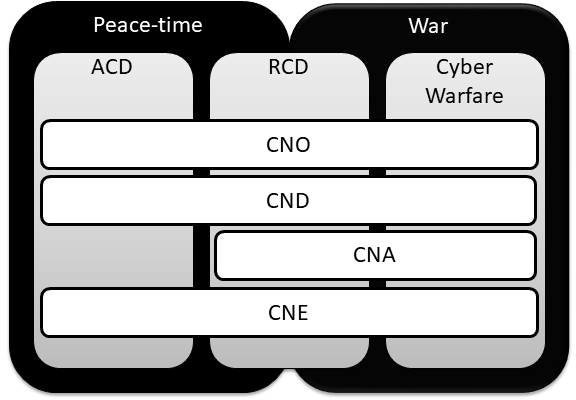
\includegraphics[width=0.5\textwidth]{./img/cno.jpg}
    \caption{Computer network operation applicability to operational paradigms}
    \label{fig:cno}
\end{figure}

% CNO requirements
Based on the related work, as presented in the chapter \ref{sec:cno-work} and discussed here, the \gls{cno} has at least the following requirements and characteristics:
\begin{enumerate}
    \item \textbf{Hybrid.} \gls{cno} can be used to aid both defensive and offensive effects as well as any other activities in support for achieving these effects.
    \item \textbf{Rapid.} Ability to deliver fast paced operation execution if such capability is prepared and maintained.
    \item \textbf{Focused.} Possibility to achieve rapid concentration of force in cyberspace on single or a small set of targets.
    \item \textbf{Dynamic.} Capability to adjust, evolve, and mutate according to the changing environment and operational needs to provide inconsistency.
    \item \textbf{Agile.} Possesses high manoeuvrability supported by the dynamic nature.
    \item \textbf{Stealthy.} Granting limited attribution, protection of identity and privileges.
    \item \textbf{Pervasive.} Has long operational reach and can target any interconnected node remotely in the cyberspace to provide access and control.
    \item \textbf{Parallel and distributed.} Can be launched from multiple sources in the cyberspace simultaneously against a single or a set of targets.
    \item \textbf{Effective.} Has the potential capability of delivering cyber and, if designated -- kinetic effects.
    \item \textbf{Asymmetric.} Can deliver higher operational effect in contrast to other operations, if prepared and used accordingly.
\end{enumerate}
This is not an exhaustive list and more characteristics could be applicable depending on the particular \gls{cno} specifics.